\documentclass{scrreprt}
\usepackage{listings}
\usepackage{underscore}
\usepackage[T2A]{fontenc}
\usepackage[utf8]{inputenc}
\usepackage[russian]{babel}
\date{}
\usepackage{geometry}
\usepackage{graphicx}
\usepackage{array}
\usepackage{tabularx}	
\usepackage{enumitem}
\usepackage{graphicx}
\usepackage{subcaption}
\usepackage{verbatim}


\geometry{
	a4paper,
	left=30mm,
	right=15mm,
	top=20mm,
	bottom=20mm
}

\usepackage{hyperref}
\begin{document}
	\begin{center}
		\textbf{Министерство науки и высшего образования Российской Федерации} \\
		\textbf{Федеральное государственное автономное образовательное учреждение высшего} \\
		\textbf{образования} \\
		«Национальный исследовательский университет ИТМО» \\
		
		\vspace{1cm}
		
		\textbf{Факультет Программной инженерии и компьютерной техники} \\
		
		\vspace{2cm}
		
		\textbf{Лабораторная работа №2} \\
		
		\vspace{1cm}
		
		по дисциплине «Основы программной инженерии» \\
		
		\vspace{1cm}
		
		Вариант: 901425 \\
		
		\vspace{2cm}
		
		\begin{flushright}
			\textbf{Преподаватель:} \\
			Карташев Владимир Сергеевич \\
			
			\vspace{0.5cm}
			
			\textbf{Выполнил:} \\
			Ребрый Егор Сергеевич \\
			
			\vspace{0.5cm}
			
			\textbf{Группа:} \\
			Р3209 \\
		\end{flushright}
		
		\vfill
		
		Санкт-Петербург, 2025 \\
	\end{center}
	
	\tableofcontents
	
	\chapter{Задание}
	
	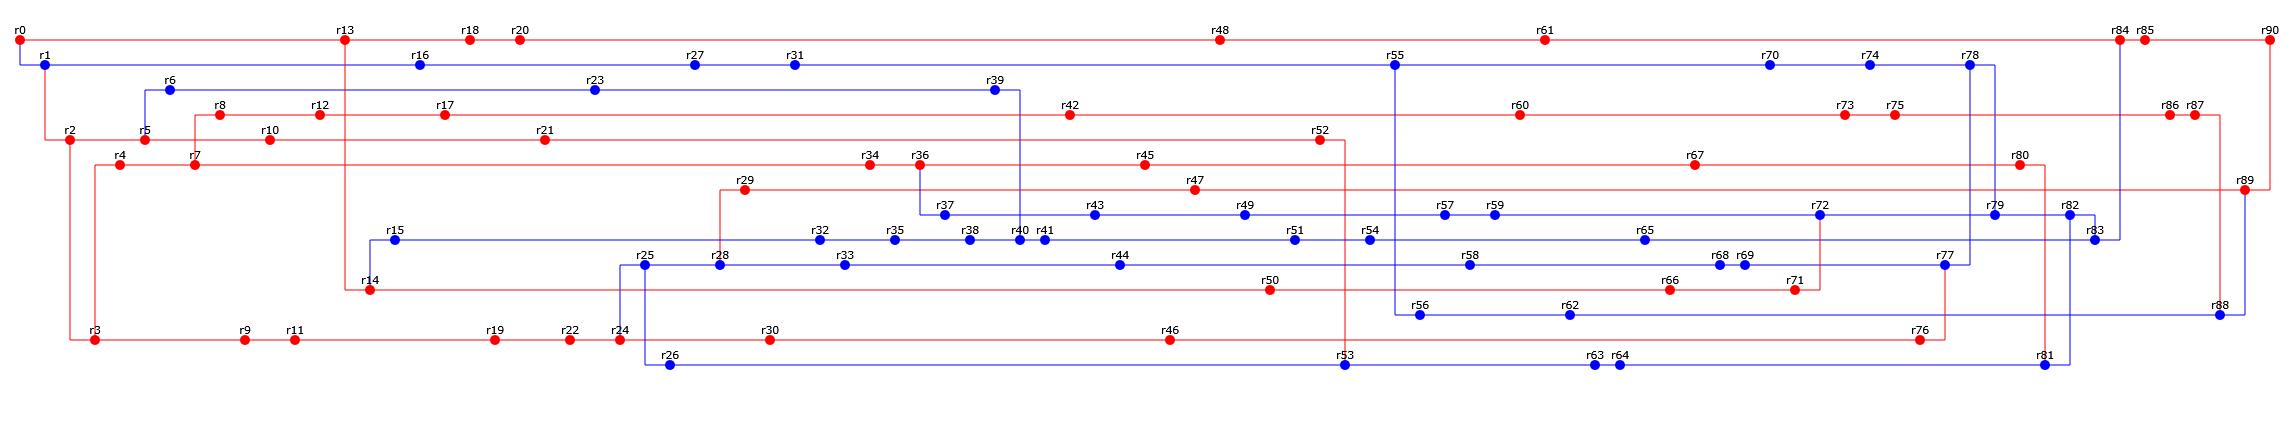
\includegraphics[width=\textwidth]{task.png}
	 Сконфигурировать в своём домашнем каталоге репозитории svn и git и загрузить в них начальную ревизию файлов с исходными кодами (в соответствии с выданным вариантом).
	
	Воспроизвести последовательность команд для систем контроля версий svn и git, осуществляющих операции над исходным кодом, приведённые на блок-схеме.
	
	При составлении последовательности команд необходимо учитывать следующие условия:
	\begin{itemize}
	\item Цвет элементов схемы указывает на пользователя, совершившего действие (красный - первый, синий - второй).
	\item Цифры над узлами - номер ревизии. Ревизии создаются последовательно.
	\item Необходимо разрешать конфликты между версиями, если они возникают.
	\end{itemize}
	\chapter{Реализация с использованием Git}
	\begin{verbatim}
		#/bin/bash
		
		USER_NAME = $(git config user.name)
		
		red() {
			git config --local user.name red
			git config --local user.email red@mail.ru
		}
		
		
		blue() {
			git config --local user.name blue
			git config --local user.email blue@mail.ru
		}
		
		commit() {
			unzip -o commits/commit$1.zip -d src
			git add ./src/*
			git commit -m "Revision $1 (r$1)"
			echo "- Коммит $1 ($USER_NAME)"
		}
		
		checkout() {
			git checkout $2 $1
		}
		
		merge() {
			git merge $1 --no-commit -X
			if [ $? -ne 0 ]; then
			echo "Обнаружен конфликт при слиянии, пожалуйста разрешите конфликт"
			read -p "После разрешения конфликта выполните 'git add .' нажмите Enter"
			while git ls-files --unmerged | grep -q '^' ; do
			read -p "Обнаружены неразрешенные конфликты, разрешите их, выполните 'git add .' и  нажмите Enter"
			done
			fi
			
		}
		
		# Удаление ненужнх данных
		rm -rf .git
		rm -f .gitignore
		rm -rf ./src
		
		# Создание репозитория 
		git init
		echo "- git init"
		
		red
		echo "- user red created"
		
		checkout master -b
		
		# Новый .gitignore {
			echo "commits" >> .gitignore
			echo "git.sh" >> .gitignore
			echo "svn.sh" >> .gitignore
			echo "svn" >> .gitignore
			git add .gitignore
			echo "- Новый .gitignore создан" 
			# }
		
		# Ревизия r0 (пользователь 1) {
			commit 0
			# }
		
		
		# Ревизия r1 (пользователь 2) {
			blue
			checkout branch2 -b
			commit 1
			# }
		
		# Ревизия r2 (пользователь 1)  {
			red
			checkout branch5 -b
			commit 2
			# }
		
		# Ревизия r3 (пользователь 1) {
			checkout branch13 -b
			commit 3
			# }
		
		# Ревизия r4 (пользователь 1) {
			checkout branch6 -b
			commit 4
			# }
		
		# Ревизия r5 (пользователь 1) {
			checkout branch5
			commit 5
			# }
		
		# Ревизия r6 (пользователь 2) {
			blue
			checkout branch3 -b
			commit 6
			# }
		
		# Ревизия r7 (пользователь 1) {
			red
			checkout branch6
			commit 7
			# }
		
		# Ревизия r8 (пользователь 1) {
			checkout branch4 -b
			commit 8
			# }
		
		# Ревизия r9 (пользователь 1) {
			checkout branch13
			commit 9
			# }
		
		# Ревизия r10 (пользователь 1) {
			checkout branch5
			commit 10
			# }
		
		# Ревизия r11 (пользователь 1) {
			checkout branch13
			commit 11
			# }
		
		# Ревизия r12 (пользователь 1) {
			checkout branch4
			commit 12
			# }
		
		# Ревизия r13 (пользователь 1) {
			checkout master
			commit 13
			# }
		
		# Ревизия r14 (пользователь 1) {
			checkout branch11 -b
			commit 14
			# }
		
		# Ревизия r15 (пользователь 2) {
			blue
			checkout branch9 -b
			commit 15
			# }
		
		# Ревизия r16 (пользователь 2) {
			checkout branch2
			commit 16
			# }
		
		# Ревизия r17 (пользователь 1) {
			red
			checkout branch4
			commit 17
			# }
		
		# Ревизия r18 (пользователь 1) {
			checkout master
			commit 18
			# }
		
		# Ревизия r19 (пользователь 1) {
			checkout branch13
			commit 19
			# }
		
		# Ревизия r20 (пользователь 1) {
			checkout master
			commit 20
			# }
		
		# Ревизия r21 (пользователь 1) {
			checkout branch5
			commit 21
			# }
		
		# Ревизия r22 (пользователь 1) {
			checkout branch13
			commit 22
			# }
		
		# Ревизия r23 (пользователь 2) {
			blue
			checkout branch3
			commit 23
			# }
		
		# Ревизия r24 (пользователь 1) {
			red
			checkout branch13
			commit 24
			# }
		
		# Ревизия r25 (пользователь 2) {
			blue
			checkout branch10 -b
			commit 25
			# }
		
		# Ревизия r26 (пользователь 2) {
			checkout branch14 -b
			commit 26
			# }
		
		# Ревизия r27 (пользователь 2) {
			checkout branch2
			commit 27
			# }
		
		# Ревизия r28 (пользователь 2) {
			checkout branch10
			commit 28
			# }
		
		# Ревизия r29 (пользователь 1) {
			red
			checkout branch7 -b
			commit 29
			# }
		
		# Ревизия r30 (пользователь 1) {
			checkout branch13
			commit 30
			# }
		
		# Ревизия r31 (пользователь 2) {
			checkout branch2
			commit 31
			# }
		
		# Ревизия r32 (пользователь 2) {
			checkout branch9
			commit 32
			# }
		
		# Ревизия r33 (пользователь 2) {
			checkout branch10
			commit 33
			# }
		
		# Ревизия r34 (пользователь 1) {
			red
			checkout branch6
			commit 34
			# }
		
		# Ревизия r35 (пользователь 2) {
			blue
			checkout branch9
			commit 35
			# }
		
		# Ревизия r36 (пользователь 1) {
			red
			checkout branch6
			commit 36
			# }
		
		# Ревизия r37 (пользователь 2) {
			blue
			checkout branch8 -b
			commit 37
			# }
		
		# Ревизия r38 (пользователь 2) {
			checkout branch9
			commit 38
			# }
		
		# Ревизия r39 (пользователь 2) {
			checkout branch3
			commit 39
			# }
		
		# Ревизия r40-r41 (пользователь 2) {
			checkout branch9
			merge branch3
			commit 40
			commit 41
			# }
		
		# Ревизия r42 (пользователь 1) {
			red 
			checkout branch4
			commit 42
			# }
		
		# Ревизия r43 (пользователь 2) {
			blue
			checkout branch8
			commit 43
			# }
		
		# Ревизия r44 (пользователь 2) {
			checkout branch10
			commit 44
			# }
		
		# Ревизия r45 (пользователь 1) {
			red
			checkout branch6
			commit 45
			# }
		
		# Ревизия r46 (пользователь 1) {
			checkout branch13
			commit 46
			# }
		
		# Ревизия r47 (пользователь 1) {
			checkout branch7
			commit 47
			# }
		
		# Ревизия r48 (пользователь 1) {
			checkout master
			commit 48
			# }
		
		# Ревизия r49 (пользователь 2) {
			blue
			checkout branch8
			commit 49
			# }
		
		# Ревизия r50 (пользователь 1) {
			red
			checkout branch11
			commit 50
			# }
		
		# Ревизия r51 (пользователь 2) {
			blue
			checkout branch9
			commit 51
			# }
		
		# Ревизия r52 (пользователь 1) {
			red
			checkout branch5
			commit 52
			# }
		
		# Ревизия r53 (пользователь 2) {
			blue
			checkout branch14
			merge branch5
			commit 53
			# }
		
		# Ревизия r54 (пользователь 2) {
			checkout branch9
			commit 54
			# }
		
		# Ревизия r55 (пользователь 2) {
			checkout branch2
			commit 55
			# }
		
		# Ревизия r56 (пользователь 2) {
			checkout branch12 -b
			commit 56
			# }
		
		# Ревизия r57 (пользователь 2) {
			checkout branch8
			commit 57
			# }
		
		# Ревизия r58 (пользователь 2) {
			checkout branch10
			commit 58
			# }
		
		# Ревизия r59 (пользователь 2) {
			checkout branch8
			commit 59
			# }
		
		# Ревизия r60 (пользователь 1) {
			red
			checkout branch4
			commit 60
			# }
		
		# Ревизия r61 (пользователь 1) {
			checkout master
			commit 61
			# }
		
		# Ревизия r62 (пользователь 2) {
			blue
			checkout branch12
			commit 62
			# }
		
		# Ревизия r63-r64 (пользователь 2) {
			checkout branch14
			commit 63
			commit 64
			# }
		
		# Ревизия r65 (пользователь 2) {
			checkout branch9
			commit 65
			# }
		
		# Ревизия r66 (пользователь 1) {
			red
			checkout branch11
			commit 66
			# }
		
		# Ревизия r67 (пользователь 1) {
			checkout branch6
			commit 67
			# }
		
		# Ревизия r68-r69 (пользователь 2) {
			blue
			checkout branch10
			commit 68
			commit 69
			# }
		
		# Ревизия r70 (пользователь 2) {
			checkout branch2
			commit 70
			# }
		
		# Ревизия r71 (пользователь 1) {
			red
			checkout branch11
			commit 71
			# }
		
		# Ревизия r72 (пользователь 2) {
			blue
			checkout branch8
			merge branch11
			commit 72
			# }
		
		# Ревизия r73 (пользователь 1) {
			red
			checkout branch4
			commit 73
			# }
		
		# Ревизия r74 (пользователь 2) {
			blue
			checkout branch2
			commit 74
			# }
		
		# Ревизия r75 (пользователь 1) {
			red
			checkout branch4
			commit 75
			# }
		
		# Ревизия r76 (пользователь 1) {
			checkout branch13
			commit 76
			# }
		
		# Ревизия r77 (пользователь 2) {
			blue
			checkout branch10
			merge branch13
			commit 77
			# }
		
		# Ревизия r78 (пользователь 2) {
			checkout branch2
			merge branch10
			commit 78
			# }
		
		# Ревизия r79 (пользователь 2) {
			checkout branch8
			merge branch2
			commit 79
			# }
		
		# Ревизия r80 (пользователь 1) {
			red
			checkout branch6
			commit 80
			# }
		
		# Ревизия r81 (пользователь 2) {
			blue
			checkout branch14
			merge branch6
			commit 81
			# }
		
		# Ревизия r82 (пользователь 2) {
			checkout branch8
			merge branch14
			commit 82
			# }
		
		# Ревизия r83 (пользователь 2) {
			checkout branch9
			merge branch8
			commit 83
			# }
		
		# Ревизия r84-r85 (пользователь 1) {
			red
			checkout master
			merge branch9
			commit 84
			commit 85
			# }
		
		# Ревизия r86-r87 (пользователь 1) {
			checkout branch4
			commit 86
			commit 87
			# }
		
		# Ревизия r88 (пользователь 2) {
			blue
			checkout branch12
			merge branch4
			commit 88
			# }
		
		# Ревизия r89 (пользователь 1) {
			red
			checkout branch7
			merge branch12
			commit 89
			# }
		
		# Ревизия r90 (пользователь 1) {
			checkout master
			merge branch7
			commit 90
			# }
		
		
	\end{verbatim}
	
	
	\chapter{Реализация с использованием SVN}
	
	\begin{verbatim}
		#!/bin/bash
		
		red() {
			CURRENT_USER=red
		}
		
		blue() { 
			CURRENT_USER=blue
		}
		
		commit() {
			unzip -o $COMMITS/commit$1.zip -d . >> /dev/null
			svn add * --force
			svn commit -m "Revision $1 (r$1)" --username $CURRENT_USER
			echo "- Commit r$1"
		}
		
		branch() {
			if [ "$1" = "trunk" ]; then
			svn copy $REMOTE_URL/trunk $REMOTE_URL/branches/"$2" -m "Create $2" --username $CURRENT_USER
			else
			svn copy $REMOTE_URL/branches/branch$1 $REMOTE_URL/branches/"$2" -m "Create $2" --username $CURRENT_USER	
			fi
			
		}
		
		switch() {
			if [ "$1" = "trunk" ]; then
			svn switch $REMOTE_URL/trunk
			else
			svn switch $REMOTE_URL/branches/"$1"
			fi
		}
		
		merge() {
			svn merge  $REMOTE_URL/branches/"$1"
			svn resolved *
		}
		
		# init
		rm -rf svn
		mkdir svn
		cd svn
		
		REMOTE_URL="file://$(pwd)/repo"
		COMMITS=$HOME/opi2/commits
		CURRENT_USER=red
		
		svnadmin create repo
		svn mkdir $REMOTE_URL/trunk $REMOTE_URL/branches -m "Project structure" --username $CURRENT_USER
		
		# создание рабочей копии
		svn checkout $REMOTE_URL/trunk working_copy
		cd working_copy
		
		
		# Ревизия r0 (пользователь 1) {
			unzip -o $COMMITS/commit0.zip -d .
			svn add *
			svn commit -m "Initial commit r0" --username $CURRENT_USER
			# }
		
		
		# Ревизия r1 (пользователь 2) {
			blue
			
			branch trunk branch2
			switch branch2
			commit 1
			# }
		
		# Ревизия r2 (пользователь 1) {
			red
			branch trunk branch5
			switch branch5
			commit 2
			# }
		
		# Ревизия r3 (пользователь 1) {
			branch trunk branch13
			switch branch13
			commit 3
			# }
		
		# Ревизия r4 (пользователь 1) {
			branch trunk branch6
			switch branch6
			commit 4
			# }
		
		# Ревизия r5 (пользователь 1) {
			switch branch5
			commit 5
			# }
		
		# Ревизия r6 (пользователь 2) {
			blue
			branch trunk branch3
			switch branch3
			commit 6
			# }
		
		# Ревизия r7 (пользователь 1) {
			red
			switch branch6
			commit 7
			# }
		
		# Ревизия r8 (пользователь 1) {
			branch trunk branch4
			switch branch4
			commit 8
			# }
		
		# Ревизия r9 (пользователь 1) {
			switch branch13
			commit 9
			# }
		
		# Ревизия r10 (пользователь 1) {
			switch branch5
			commit 10
			# }
		
		# Ревизия r11 (пользователь 1) {
			switch branch13
			commit 11
			# }
		
		# Ревизия r12 (пользователь 1) {
			switch branch4
			commit 12
			# }
		
		# Ревизия r13 (пользователь 1) {
			switch trunk
			commit 13
			# }
		
		# Ревизия r14 (пользователь 1) {
			branch trunk branch11
			switch branch11
			commit 14
			# }
		
		# Ревизия r15 (пользователь 2) {
			blue
			branch trunk branch9
			switch branch9
			commit 15
			# }
		
		# Ревизия r16 (пользователь 2) {
			switch branch2
			commit 16
			# }
		
		# Ревизия r17 (пользователь 1) {
			red
			switch branch4
			commit 17
			# }
		
		# Ревизия r18 (пользователь 1) {
			switch trunk
			commit 18
			# }
		
		# Ревизия r19 (пользователь 1) {
			switch branch13
			commit 19
			# }
		
		# Ревизия r20 (пользователь 1) {
			switch trunk
			commit 20
			# }
		
		# Ревизия r21 (пользователь 1) {
			switch branch5
			commit 21
			# }
		
		# Ревизия r22 (пользователь 1) {
			switch branch13
			commit 22
			# }
		
		# Ревизия r23 (пользователь 2) {
			blue
			switch branch3
			commit 23
			# }
		
		# Ревизия r24 (пользователь 1) {
			red
			switch branch13
			commit 24
			# }
		
		# Ревизия r25 (пользователь 2) {
			blue
			branch trunk branch10
			switch branch10
			commit 25
			# }
		
		# Ревизия r26 (пользователь 2) {
			branch trunk branch14
			switch branch14
			commit 26
			# }
		
		# Ревизия r27 (пользователь 2) {
			switch branch2
			commit 27
			# }
		
		# Ревизия r28 (пользователь 2) {
			switch branch10
			commit 28
			# }
		
		# Ревизия r29 (пользователь 1) {
			red
			branch trunk branch7
			switch branch7
			commit 29
			# }
		
		# Ревизия r30 (пользователь 1) {
			switch branch13
			commit 30
			# }
		
		# Ревизия r31 (пользователь 2) {
			blue
			switch branch2
			commit 31
			# }
		
		# Ревизия r32 (пользователь 2) {
			switch branch9
			commit 32
			# }
		
		# Ревизия r33 (пользователь 2) {
			switch branch10
			commit 33
			# }
		
		# Ревизия r34 (пользователь 1) {
			red
			switch branch6
			commit 34
			# }
		
		# Ревизия r35 (пользователь 2) {
			blue
			switch branch9
			commit 35
			# }
		
		# Ревизия r36 (пользователь 1) {
			red
			switch branch6
			commit 36
			# }
		
		# Ревизия r37 (пользователь 2) {
			blue
			branch trunk branch8
			switch branch8
			commit 37
			# }
		
		# Ревизия r38 (пользователь 2) {
			switch branch9
			commit 38
			# }
		
		# Ревизия r39 (пользователь 2) {
			switch branch3
			commit 39
			# }
		
		# Ревизия r40-r41 (пользователь 2) {
			switch branch9
			merge branch3
			commit 40
			commit 41
			# }
		
		# Ревизия r42 (пользователь 1) {
			red 
			switch branch4
			commit 42
			# }
		
		# Ревизия r43 (пользователь 2) {
			blue
			switch branch8
			commit 43
			# }
		
		# Ревизия r44 (пользователь 2) {
			switch branch10
			commit 44
			# }
		
		# Ревизия r45 (пользователь 1) {
			red
			switch branch6
			commit 45
			# }
		
		# Ревизия r46 (пользователь 1) {
			switch branch13
			commit 46
			# }
		
		# Ревизия r47 (пользователь 1) {
			switch branch7
			commit 47
			# }
		
		# Ревизия r48 (пользователь 1) {
			switch trunk
			commit 48
			# }
		
		# Ревизия r49 (пользователь 2) {
			blue
			switch branch8
			commit 49
			# }
		
		# Ревизия r50 (пользователь 1) {
			red
			switch branch11
			commit 50
			# }
		
		# Ревизия r51 (пользователь 2) {
			blue
			switch branch9
			commit 51
			# }
		
		# Ревизия r52 (пользователь 1) {
			red
			switch branch5
			commit 52
			# }
		
		# Ревизия r53 (пользователь 2) {
			blue
			switch branch14
			merge branch5
			commit 53
			# }
		
		# Ревизия r54 (пользователь 2) {
			switch branch9
			commit 54
			# }
		
		# Ревизия r55 (пользователь 2) {
			switch branch2
			commit 55
			# }
		
		# Ревизия r56 (пользователь 2) {
			branch trunk branch12
			switch branch12
			commit 56
			# }
		
		# Ревизия r57 (пользователь 2) {
			switch branch8
			commit 57
			# }
		
		# Ревизия r58 (пользователь 2) {
			switch branch10
			commit 58
			# }
		
		# Ревизия r59 (пользователь 2) {
			switch branch8
			commit 59
			# }
		
		# Ревизия r60 (пользователь 1) {
			red
			switch branch4
			commit 60
			# }
		
		# Ревизия r61 (пользователь 1) {
			switch trunk
			commit 61
			# }
		
		# Ревизия r62 (пользователь 2) {
			blue
			switch branch12
			commit 62
			# }
		
		# Ревизия r63-r64 (пользователь 2) {
			switch branch14
			commit 63
			commit 64
			# }
		
		# Ревизия r65 (пользователь 2) {
			switch branch9
			commit 65
			# }
		
		# Ревизия r66 (пользователь 1) {
			red
			switch branch11
			commit 66
			# }
		
		# Ревизия r67 (пользователь 1) {
			switch branch6
			commit 67
			# }
		
		# Ревизия r68-r69 (пользователь 2) {
			blue
			switch branch10
			commit 68
			commit 69
			# }
		
		# Ревизия r70 (пользователь 2) {
			switch branch2
			commit 70
			# }
		
		# Ревизия r71 (пользователь 1) {
			red
			switch branch11
			commit 71
			# }
		
		# Ревизия r72 (пользователь 2) {
			blue
			switch branch8
			merge branch11
			commit 72
			# }
		
		# Ревизия r73 (пользователь 1) {
			red
			switch branch4
			commit 73
			# }
		
		# Ревизия r74 (пользователь 2) {
			blue
			switch branch2
			commit 74
			# }
		
		# Ревизия r75 (пользователь 1) {
			red
			switch branch4
			commit 75
			# }
		
		# Ревизия r76 (пользователь 1) {
			switch branch13
			commit 76
			# }
		
		# Ревизия r77 (пользователь 2) {
			blue
			switch branch10
			merge branch13
			commit 77
			# }
		
		# Ревизия r78 (пользователь 2) {
			switch branch2
			merge branch10
			commit 78
			# }
		
		# Ревизия r79 (пользователь 2) {
			switch branch8
			merge branch2
			commit 79
			# }
		
		# Ревизия r80 (пользователь 1) {
			red
			switch branch6
			commit 80
			# }
		
		# Ревизия r81 (пользователь 2) {
			blue
			switch branch14
			merge branch6
			commit 81
			# }
		
		# Ревизия r82 (пользователь 2) {
			switch branch8
			merge branch14
			commit 82
			# }
		
		# Ревизия r83 (пользователь 2) {
			switch branch9
			merge branch8
			commit 83
			# }
		
		# Ревизия r84-r85 (пользователь 1) {
			red
			switch trunk
			merge branch9
			commit 84
			commit 85
			# }
		
		# Ревизия r86-r87 (пользователь 1) {
			switch branch4
			commit 86
			commit 87
			# }
		
		# Ревизия r88 (пользователь 2) {
			blue
			switch branch12
			merge branch4
			commit 88
			# }
		
		# Ревизия r89 (пользователь 1) {
			red
			switch branch7
			merge branch12
			commit 89
			# }
		
		# Ревизия r90 (пользователь 1) {
			switch trunk
			merge branch7
			commit 90
			# }
		
	\end{verbatim}
	
	\chapter{Вывод}
	
\end{document}